\section{ProLoSA Implementation}
\label{app:method_details}
\label{sec:method}
\subsection{{ProLoSA} Parameterization}
\label{sec:prolosa_parameterization}

Let $\mathcal{L}$ denote the set of adapted linear layers with frozen weights $W_0$.
For each $\ell\in\mathcal{L}$, LoRA introduces a low-rank update $\Delta W_\ell=B_\ell A_\ell$ with
$A_\ell\in\mathbb{R}^{r_\ell\times d_\ell^{\mathrm{in}}}$,
$B_\ell\in\mathbb{R}^{d_\ell^{\mathrm{out}}\times r_\ell}$,
and we write
$\theta_D=\mathrm{vec}(\{A_\ell,B_\ell\}_{\ell\in\mathcal{L}})\in\mathbb{R}^{D}$
for the vectorized LoRA parameters.
Instead of directly optimizing $\theta_D$, {ProLoSA} reconstructs it as (Figure~\ref{fig:framework})
\begin{equation}
\theta_D = P\theta_d + R\alpha,
\label{eq:prolosa_main}
\end{equation}
where $\theta_d\in\mathbb{R}^{d}$ is the compressed latent parameter,
$P\in\mathbb{R}^{D\times d}$ is a fixed projection matrix,
$R\in\{0,1\}^{D\times K}$ routes sparse residual coefficients to selected full-space coordinates,
and $\alpha\in\mathbb{R}^{K}$ contains the trainable sparse coefficients, for a total budget of $B=d+K$ trainable parameters with $d,K\ll D$.

\begin{figure*}[t]
\centering
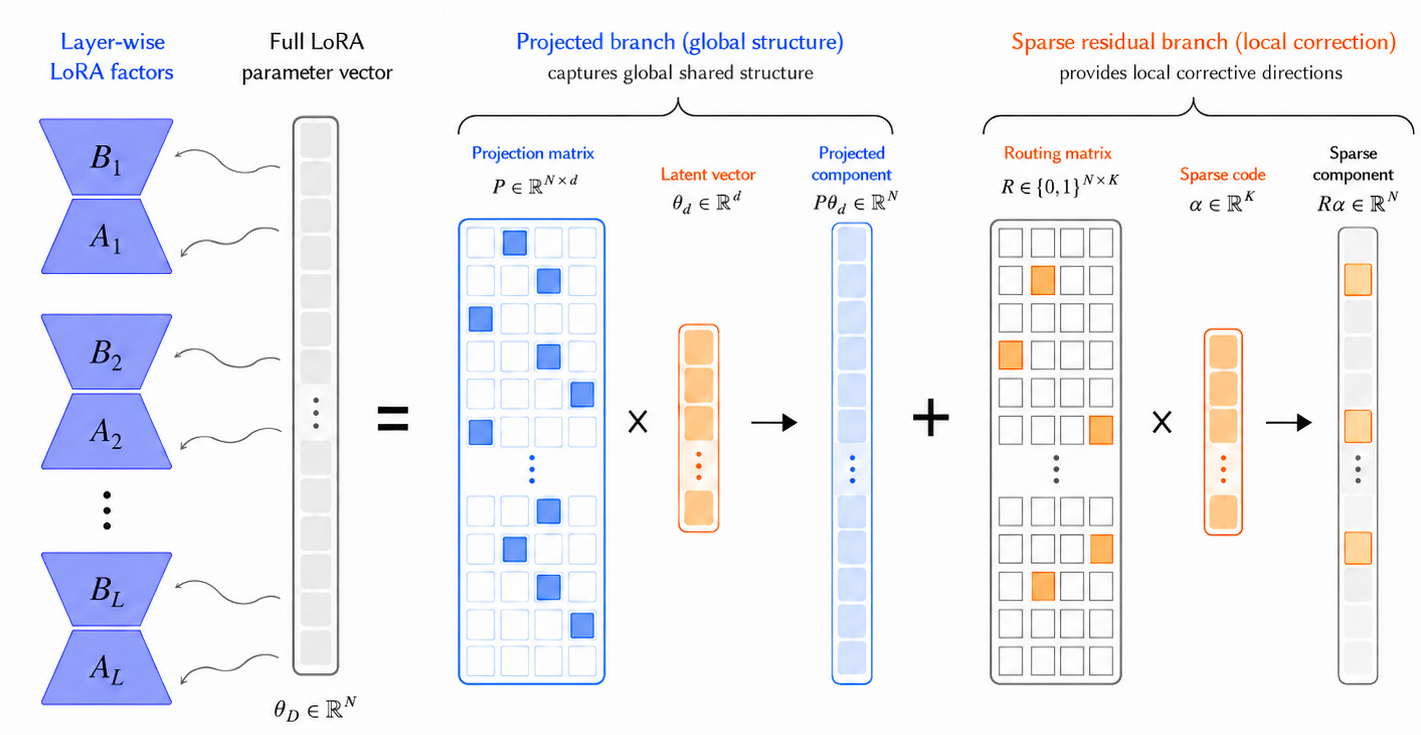
\includegraphics[width=0.65\textwidth]{framework.png}
\caption{
Overview of \textbf{ProLoSA}.
The full LoRA parameter vector is reconstructed as
$\theta_D=P\theta_d+R\alpha$, where the projected branch captures globally shared adaptation structure and the sparse residual branch restores local corrective directions on selected coordinates.
}
\label{fig:framework}
\end{figure*}

We instantiate $P$ with the normalized one-hot projection of Uni-LoRA~\citep{li2025unilora}: an assignment
$\phi:\{1,\ldots,D\}\rightarrow\{1,\ldots,d\}$, sampled once at initialization and kept fixed, maps each full-space coordinate to a latent coordinate, and
\begin{equation}
P_{ij}
=
\begin{cases}
c_j^{-1/2}, & \text{if } j=\phi(i),\\
0, & \text{otherwise},
\end{cases}
\qquad
c_j=|\{i:\phi(i)=j\}|,
\label{eq:projection_matrix_construction}
\end{equation}
so that each row of $P$ has exactly one nonzero entry and $P^\top P=I_d$.
The projected branch thus ties the $D$ LoRA coordinates into $d$ shared groups, while $R\alpha$ provides direct coordinate-wise correction on selected high-sensitivity directions.
After reconstruction, $\theta_D$ is unpacked into layer-wise factors $(A_\ell,B_\ell)$ with $\Delta W_\ell=B_\ell A_\ell$; since the final update consists of standard LoRA factors, it can be merged into the frozen backbone with no additional inference latency.

\subsection{Warmup Support Selection and Training}
\label{sec:routed_sparse_adapter}

Rather than learning a dense residual with $D$ additional parameters, {ProLoSA} activates only $K$ coordinates selected through a compressed warmup procedure, and is trained in two stages.

\emph{Stage 1: compressed warmup and support selection.}
The sparse branch is initially inactive, so $\theta_D^{(t)}=P\theta_d^{(t)}$.
Let $T$ be the total number of training steps and $\rho_{\mathrm{w}}$ the warmup ratio.
Only $\theta_d$ is optimized during the first $T_{\mathrm{pre}}=\lfloor\rho_{\mathrm{w}}T\rfloor$ steps; the model then continues to optimize $\theta_d$ for a fixed window of $T_{\mathrm{s}}=128$ steps while accumulating a SNIP-style sensitivity score~\citep{lee2018snip,he2022sparseadapter} for each full-space coordinate,
\begin{equation}
s_i
=
\sum_{t=T_{\mathrm{pre}}+1}^{T_{\mathrm{pre}}+T_{\mathrm{s}}}
\left|
\theta_{D,i}^{(t)}
g_i^{(t)}
\right|,
\qquad
g^{(t)}=\nabla_{\theta_D^{(t)}}\mathcal{L}^{(t)},
\label{eq:warmup_snip_score}
\end{equation}
which measures the accumulated first-order effect of perturbing coordinate $i$ (see Appendix~\ref{app:warmup_snip} for the derivation).
Note that the sparse branch is activated only after $T_{\mathrm{pre}}+T_{\mathrm{s}}$ steps in total: the warmup ratio $\rho_{\mathrm{w}}$ parameterizes only the score-free phase, so the compressed-only stage lasts $\lfloor\rho_{\mathrm{w}}T\rfloor+128$ steps, slightly longer than $\rho_{\mathrm{w}}T$.
The score $s_i$ is a practical \emph{proxy} for the quantity the theory asks for---the curvature-weighted off-subspace residual energy of coordinate $i$ (Appendices~\ref{sec:sparse_bias} and Appendix~\ref{app:isotropic_bias_reduction})---rather than that quantity itself: since $\theta_D=P\theta_d$ during warmup, coordinates tied to the same latent entry share the same value and are distinguished by their gradients, which reflect functional sensitivity.
Whether this proxy actually concentrates on high-energy off-subspace directions is an empirical question that experiment E5 (Appendix~\ref{sec:real_model_validation}) tests directly by measuring the captured-energy enrichment of the selected support.

\emph{Stage 2: joint training on a fixed support.}
{ProLoSA} selects the top-$K$ coordinates $\mathcal{I}=\operatorname{TopK}(\{s_i\}_{i=1}^{D},K)$, constructs $R=[e_{i_1},\ldots,e_{i_K}]$, and initializes $\alpha=0$ so that activating the residual branch does not abruptly change $\theta_D$.
Thereafter, $\theta_d$ and $\alpha$ are jointly optimized under Eq.~\eqref{eq:prolosa_main} by minimizing the downstream training loss with the backbone $W_0$ frozen, while $P$ and $R$ remain fixed.
The fixed support avoids the instability of a changing parameterization while allocating extra capacity to coordinates identified as highly sensitive after initial compressed adaptation; after training, the update is merged into the backbone as in standard LoRA.
The full procedure is summarized in Appendix~\ref{app:algorithm} (Algorithm~\ref{alg:prolosa}).

\subsection{Connection to Warmup SNIP Support Selection}
\label{app:warmup_snip}

The analysis above holds for any fixed sparse support $I$.
In practice, ProLoSA selects this support using sensitivity scores accumulated during the final fixed window of a compressed warmup stage.
Specifically, the compressed branch is first optimized for
$T_{\mathrm{pre}}=\lfloor\rho_{\mathrm{w}}T\rfloor$
steps without accumulating support-selection scores.
It is then further optimized for a fixed sensitivity-score accumulation window of
$T_{\mathrm{s}}=128$ steps, so the sparse branch is activated after $T_{\mathrm{pre}}+T_{\mathrm{s}}$ steps in total.
Throughout the warmup stage, the sparse branch is inactive and the reconstructed LoRA parameter vector is
\begin{equation}
\theta_D^{(t)}=P\theta_d^{(t)} .
\label{eq:app_warmup_reconstruction}
\end{equation}

Consider perturbing coordinate $i$ of $\theta_D^{(t)}$.
A first-order Taylor approximation of the mini-batch loss gives
\begin{equation}
\begin{aligned}
\mathcal{L}^{(t)}(\theta_D^{(t)}+\delta_i e_i)
-
\mathcal{L}^{(t)}(\theta_D^{(t)})
&\approx
g_i^{(t)}\delta_i, \\
g^{(t)}
&=
\nabla_{\theta_D^{(t)}}\mathcal{L}^{(t)} .
\end{aligned}
\label{eq:app_first_order_perturbation}
\end{equation}

Following SNIP-style saliency criteria, we measure the sensitivity of coordinate $i$ by the first-order effect of removing or perturbing its current value.
Setting $\delta_i=-\theta_{D,i}^{(t)}$ gives
\begin{equation}
\left|
\theta_{D,i}^{(t)}g_i^{(t)}
\right|.
\label{eq:app_single_step_snip_score}
\end{equation}

Accumulating this quantity over the fixed sensitivity-score accumulation window yields
\begin{equation}
s_i
=
\sum_{t=T_{\mathrm{pre}}+1}^{T_{\mathrm{pre}}+T_{\mathrm{s}}}
\left|
\theta_{D,i}^{(t)}g_i^{(t)}
\right|,
\qquad
T_{\mathrm{s}}=128.
\label{eq:app_warmup_snip_score}
\end{equation}

Coordinates with large $s_i$ are those whose perturbation has a consistently large first-order effect on the training loss during this compressed adaptation window.
Selecting the top-$K$ coordinates therefore provides a data-dependent heuristic for identifying directions where the compressed branch may require local correction.
This support-selection rule does not guarantee the globally optimal support in the theoretical sense, but it aligns the sparse residual budget with coordinates that are locally influential during the final fixed window of the compressed warmup trajectory.


\subsection{Training Algorithm}
\label{app:algorithm}

Algorithm~\ref{alg:prolosa} summarizes the full training procedure of {ProLoSA}.
The first stage performs compressed-only training for $T_{\mathrm{pre}}+T_{\mathrm{s}}$ steps, with coordinate-wise sensitivity scores accumulated only during the final fixed $T_{\mathrm{s}}=128$-step window; the warmup ratio $\rho_{\mathrm{w}}$ determines only $T_{\mathrm{pre}}=\lfloor\rho_{\mathrm{w}}T\rfloor$, so the sparse branch is activated at step $\lfloor\rho_{\mathrm{w}}T\rfloor+128$ rather than at exactly $\rho_{\mathrm{w}}T$.
The second stage fixes the selected sparse support and jointly optimizes the projected and sparse residual branches.

\begin{algorithm}[!htbp]
\small
\caption{{ProLoSA} with Warmup SNIP Support Selection}
\label{alg:prolosa}
\begin{algorithmic}[1]
\REQUIRE Frozen backbone $W_0$; projection matrix $P$; sparse budget $K$; warmup ratio $\rho_{\mathrm{w}}$; sensitivity-score accumulation steps $T_{\mathrm{s}}=128$; total training steps $T$.
\STATE Initialize compressed latent parameter $\theta_d$.
\STATE Set sparse adapter inactive and initialize score vector $s \leftarrow 0_D$.
\STATE Set $T_{\mathrm{pre}}\leftarrow\lfloor\rho_{\mathrm{w}}T\rfloor$.
\FOR{$t=1$ to $T_{\mathrm{pre}}$}
    \STATE Reconstruct $\theta_D^{(t)} \leftarrow P\theta_d^{(t)}$ and unpack it into $\{A_\ell,B_\ell\}_{\ell\in\mathcal{L}}$.
    \STATE Compute mini-batch loss $\mathcal{L}^{(t)}$.
    \STATE Update $\theta_d$ by back-propagation.
\ENDFOR
\FOR{$t=T_{\mathrm{pre}}+1$ to $T_{\mathrm{pre}}+T_{\mathrm{s}}$}
    \STATE Reconstruct $\theta_D^{(t)} \leftarrow P\theta_d^{(t)}$ and unpack it into $\{A_\ell,B_\ell\}_{\ell\in\mathcal{L}}$.
    \STATE Compute mini-batch loss $\mathcal{L}^{(t)}$ and gradient $g^{(t)} \leftarrow \nabla_{\theta_D^{(t)}}\mathcal{L}^{(t)}$.
    \STATE Accumulate scores $s \leftarrow s+\left|\theta_D^{(t)}\odot g^{(t)}\right|$.
    \STATE Update $\theta_d$ by back-propagation.
\ENDFOR
\STATE Select sparse support $\mathcal{I}\leftarrow\operatorname{TopK}(s,K)$.
\STATE Construct $R=[e_{i_1},\ldots,e_{i_K}]$ for $\mathcal{I}=\{i_1,\ldots,i_K\}$ and initialize $\alpha\leftarrow 0$.
\FOR{$t=T_{\mathrm{pre}}+T_{\mathrm{s}}+1$ to $T$}
    \STATE Reconstruct $\theta_D \leftarrow P\theta_d+R\alpha$ and unpack it into $\{A_\ell,B_\ell\}_{\ell\in\mathcal{L}}$.
    \STATE Compute mini-batch loss $\mathcal{L}^{(t)}$.
    \STATE Update $\theta_d$ and $\alpha$ by back-propagation.
\ENDFOR
\RETURN Trained $\theta_d$, $\alpha$, and fixed routing matrix $R$.
\end{algorithmic}
\end{algorithm}


